\section{Pattern mining}\label{sec:m4}

\subsection{Transactional encoding}\label{sec:enc}
Each seller becomes a transaction with at most one item per attribute, written \emph{attribute=value}:
\begin{itemize}
\item \textbf{Equal-frequency tertiles} (\emph{low}/\emph{mid}/\emph{high}) for seven skewed attributes: size, price, mileage, days on market (\emph{dom}), horsepower (\emph{hp}), listing span, share of ex-taxis (\emph{cab}). Equal-width bins would put almost all sellers in one bin.
\item \textbf{Domain bins} for savings: \emph{none} (37\% exact zeros), and \emph{low}/\emph{high} split at the median of the positive values.
\item \textbf{Presence items} \emph{salvage=yes} and \emph{theft=yes} for the zero-inflated shares.
\item The grouped categoricals (body, colour, transmission, dealer, inventory) and \emph{rating}.
\end{itemize}
Missing values simply produce no item. Items with support above 0.9 (\emph{trans=a}, 94\%) are removed: they would double every pattern with lift $\approx1$. The result is 50 items and 13.3 items per seller, a dense dataset. Bin edges are learned on the data being mined: all sellers for description (\cref{sec:freq,sec:rules}), training folds only for prediction (\cref{sec:exploit}). We used Apriori; the available FP-Growth implementation returns the same itemsets but was about 70 times slower with so few and dense items.

\subsection{Frequent itemsets}\label{sec:freq}
\begin{figure*}[t]
\centering
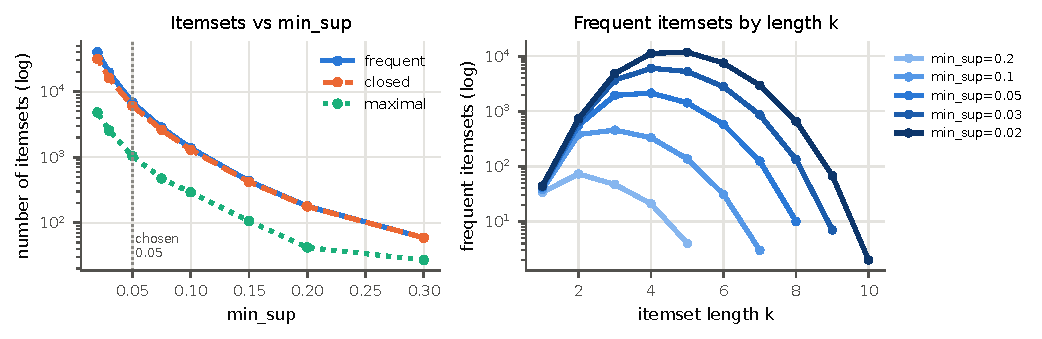
\includegraphics[width=0.93\textwidth]{m4_itemsets_sweep}
\caption{Number of frequent, closed and maximal itemsets vs \code{min\_sup} (left) and frequent itemsets by length $k$ (right).}\label{fig:isets}
\end{figure*}

\begin{table}[t]
\centering
\caption{Itemsets by \code{min\_sup} (all tested values).}\label{tab:isets}
\tab{m4_sweep}
\end{table}

\paragraph{Quantitative analysis} The number of itemsets grows about exponentially as \code{min\_sup} decreases (\cref{fig:isets,tab:isets}) and the mode of the length distribution moves from $k=2$ at 0.2 to $k=5$ at 0.02: tertile items all have support near 1/3, so long conjunctions of typical values stay frequent. Closed itemsets are 79--100\% of the frequent ones, i.e.\ few items imply each other exactly; maximal ones are 5--8 times fewer at \code{min\_sup}$\,\leq0.1$. We chose \textbf{\code{min\_sup}$\,=0.05$} (6\,835 itemsets, 1\,042 maximal): every pattern describes at least 693 sellers, \emph{rating=low} (18.6\%) can still combine with other items, and lower values multiply the output by 3--6 with mostly redundant combinations.

\paragraph{Qualitative analysis} \Cref{tab:iset} shows the most frequent closed itemsets with at least four items, and the most frequent ones containing each rating. Two seller types emerge without any distance: the \emph{franchise new-car dealer} (31\%) and the \emph{independent budget used-car dealer} (30\%), the K-Means segments C0 and C3. The longest maximal itemset (8 items, 7.7\%) refines the former with SUV, high price, large size and \emph{rating=medium}. Among the ratings, \emph{high} occurs mostly with independent used-car sellers, \emph{low} with mixed-inventory franchises; their lift decides whether this exceeds chance.

\begin{table}[t]
\centering
\caption{Most frequent closed itemsets with $k\geq4$ (top), and with a rating item and $k\geq3$ (bottom).}\label{tab:iset}
\tab{m4_itemsets}
\end{table}

\subsection{Association rules}\label{sec:rules}
\paragraph{Quantitative analysis} From the 0.05-frequent itemsets we generated 87\,266 rules with confidence at least 0.3 and counted them for eight \code{min\_conf} values and every length (\cref{fig:rules}). Counts peak at $k=5$, since an itemset of size $k$ yields $2^k-2$ rules, and fall slowly: only 12.5 times from \code{min\_conf} 0.3 to 0.95, because the encoding contains near-deterministic relations (6\,971 rules have confidence $\geq0.95$). We chose \textbf{\code{min\_conf}$\,=0.6$}: 34\,233 rules remain and 99.8\% of them have lift above 1 (100\% from 0.7), so confidences that only reflect a frequent consequent are excluded. The confidence histogram is spread over $[0.6,1]$ (median 0.78) with a peak at 1. Lift concentrates between 2 and 3 (median 2.2): a tertile consequent caps it at 3, and the tail up to 6.4 comes from multi-item consequents. High confidence occurs at every support, high lift only at low support.

\begin{figure*}[t]
\centering
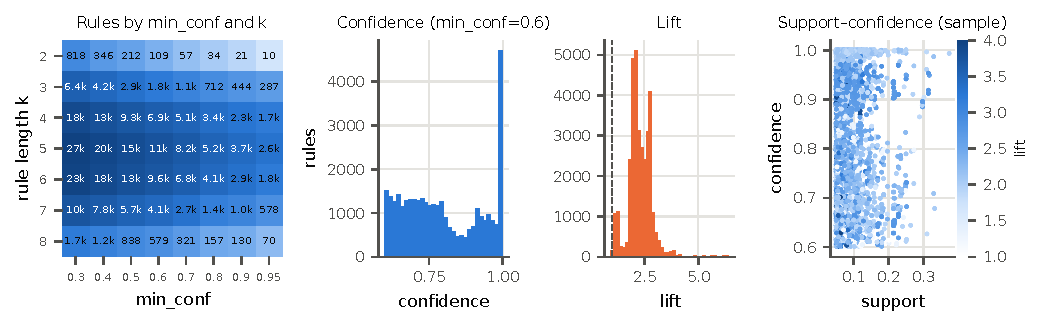
\includegraphics[width=0.97\textwidth]{m4_rules_quant}
\caption{Association rules: counts by \code{min\_conf} and length $k$; histograms of confidence and lift for \code{min\_conf}$\,=0.6$; support--confidence--lift scatter (6\,000 sampled rules).}\label{fig:rules}
\end{figure*}

\paragraph{Qualitative analysis} Ranking by lift alone returns dozens of variants of the same rule. We keep single-item consequents, drop a rule when a subset of its antecedent reaches 99\% of its lift, and show the best rule per consequent (\cref{tab:rules}). They describe inventories and agree with the regressions of \cref{sec:reg}: price, power and mileage determine each other; CVT gearboxes go with small engines; discounting franchises sell mid-mileage cars; franchises with theft-title vehicles are the large ones (more cars, more chance to have one).

\begin{table}[t]
\centering
\caption{Best rule for each consequent, by lift (\code{min\_sup}$\,=0.05$, \code{min\_conf}$\,=0.6$).}\label{tab:rules}
\tabtight{m4_rules}
\end{table}

\paragraph{Rating rules} No rule with consequent \emph{rating=low} or \emph{high} reaches confidence 0.6, so we mined them apart (\code{min\_sup}$\,=0.01$, at most three antecedent items; \cref{tab:rating}). \emph{High} is predicted by small sellers with mid-priced or mid-mileage stock (confidence 0.54 against a base rate of 0.27), \emph{low} by large sellers with mid-priced sedans, CVT or low-power cars (0.40 vs 0.19), \emph{medium} by large expensive sellers (0.77 vs 0.55). Supports are 1--2\% and no rule for \emph{low} or \emph{high} exceeds 0.55 confidence.

\begin{table}[t]
\centering
\caption{Top rating rules by lift (\code{min\_sup}$\,=0.01$).}\label{tab:rating}
\tabtight{m4_rating}
\end{table}

\paragraph{Sensitivity to binning} \Cref{tab:bin} repeats mining and a smaller rule classifier ($s=0.01$, $L=3$, training folds only) under six binnings. Equal-width bins fail, as argued in \cref{sec:enc}: one bin holds up to 100\% of the sellers, lift shrinks and the classifier falls to 0.26--0.29. Two bins triple the itemsets with less specific patterns. Four equal-frequency bins predict better than three (0.420 vs 0.390) with half the itemsets: a possible improvement that we did not tune further, because it was found after the test set had been read. We keep tertiles, whose \emph{low}/\emph{mid}/\emph{high} labels are readable in all descriptive rules.

\begin{table*}[t]
\centering
\caption{Binning sensitivity (without rating items): items, itemsets at \code{min\_sup}$\,=0.05$, rules at \code{min\_conf}$\,=0.6$ and their lift, largest support of a numerical bin, and CV macro-F1 of the rule classifier ($s=0.01$, $L=3$).}\label{tab:bin}
\tabwide{m5_binning}
\end{table*}

\subsection{Exploiting the rules}\label{sec:exploit}
\paragraph{Predicting the rating} The classifier uses the split of \cref{sec:m3}; edges, items and rules come from training data only and hyperparameters from the same 5 folds, with re-mining inside each. Every frequent antecedent $A$ (no rating items) carries the class distribution $P(c\mid A)$ of the sellers it matches, i.e.\ the confidences of its three rules. The delicate choice is how to combine matching rules. We compared eight aggregations over $s\in\{0.005,0.01,0.02\}$ and antecedent length $L\leq4$ (96 configurations, \cref{tab:agg}):
\begin{itemize}
\item \emph{class-best-conf/lift} (CBA style): best matching rule with lift $>1$ per class, then argmax;
\item \emph{best-antecedent}: the matching antecedent with the highest lift, which predicts its most confident class;
\item \emph{top10}, \emph{mean}: average $P(c\mid A)$ over the ten most discriminative, or all, matching antecedents;
\item \emph{+ prior}: the same, divided by $P(c)$.
\end{itemize}

\begin{table*}[t]
\centering
\caption{Rule-based classifier, CV macro-F1 for all 96 configurations (leading zero omitted).}\label{tab:agg}
\tabwide{m4_agg}
\end{table*}

\begin{figure*}[t]
\centering
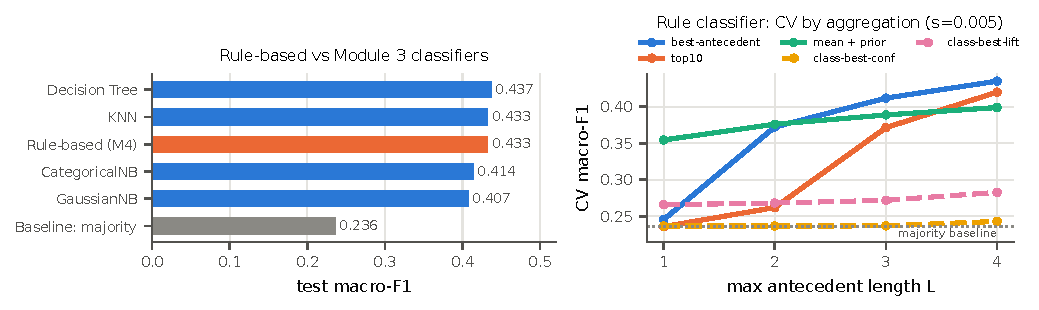
\includegraphics[width=0.93\textwidth]{m4_rule_classifier}
\caption{Test macro-F1 of the rule-based and the \cref{sec:m3} baseline-grid classifiers (left); effect of aggregation and antecedent length in CV (right).}\label{fig:rulecls}
\end{figure*}

The aggregation matters more than any other parameter. Per-class maxima fail (0.24--0.28) because they are not comparable: confidence is bounded by class frequency, so \emph{medium} always wins, and lift by $1/P(c)$, which favours \emph{low}. \emph{best-antecedent} avoids this since its three confidences come from the same sellers: $s=0.005$, $L=4$ gives CV macro-F1 0.435, growing with $L$ (\cref{fig:rulecls}, right). On the test set it reaches macro-F1 0.433 and accuracy 0.492 with 100\% coverage: equal to the Decision Tree (0.437) and KNN (0.433) of the baseline grid, with more weight on \emph{medium} (recall 0.58) and less on \emph{low} (0.25). The model holds 46k rules and is not readable as a whole, but every single prediction is explained by one rule.

\paragraph{Generalization of the rules} Ranking thousands of rules by lift selects lucky ones. We took the 50 rating rules with the highest training lift in each support band and re-measured them on the test set (\cref{tab:gen}; \cref{fig:cross}, right). In every band they remain positively associated on average, but the excess over 1 shrinks, most where support is lowest: by 28\% for \emph{low} and 49\% for \emph{medium} at 0.5--1\%, against 3--10\% for \emph{high} above 1\%. Extreme lifts at low support are partly selection, so a rule should be judged on support too.

\begin{table}[t]
\centering
\caption{Mean lift of the 50 best rating rules per support band, training $\to$ test.}\label{tab:gen}
\tabtight{m5_gen}
\end{table}

\paragraph{Imputing missing values} We masked an attribute for all 2\,769 test sellers and predicted it with the most confident matching rule mined on the training set (\code{min\_sup}$\,=0.01$, at most three antecedent items, rating excluded). \Cref{tab:imp}: the \textbf{price tertile} is recovered in 75.2\% of the cases against 35.1\% for the mode; the \textbf{body type} is not (65.0\% vs 64.2\%), because its determinants, the dimensions, are not encoded as items. Rules impute well exactly when the transactions contain the drivers of the attribute.

\begin{table}[t]
\centering
\caption{Rule-based imputation of masked test values.}\label{tab:imp}
\tabtight{m4_imp}
\end{table}

\subsection{Describing the segments with rules}\label{sec:segrules}
Adding the K-Means segment as an item and mining $A\to$ \emph{segment} (\code{min\_sup}$\,=0.02$) gives short definitions of the clusters (\cref{tab:segrules}). C0, C1 and C3 are almost deterministic (confidence $\geq0.97$). C2 needs slow turnover \emph{and} a long span and stays at 0.84, with lift 9: the same fragility found with DBSCAN. With these rules a seller can be assigned to a segment without computing distances.

\begin{table}[t]
\centering
\caption{Two most confident non-redundant rules per K-Means segment.}\label{tab:segrules}
\tabtight{m4_segments}
\end{table}
